\documentclass[master=ucll,dutch,twoside]{ucllfilip}
%\documentclass[master=bin,masteroption=eg]{kulemt}
%master is hetgene dat gedefinieerd staat in de .cfg file
%masteroption is hetgene bij ELT gedeelte staat als optie
%and command is voor een 2de lijn bij te voegen
\setup{
	title={Samenvatting Distributed Applications},
  author={Filip Vanden Eynde \and R0363898 \and 3TX/1},
  promotor={Professor Kasper Cools}}



% De volgende \ setup mag verwijderd worden als geen fiche gewenst is.
\setup{filingcard,
  translatedtitle={Portfolio money management},
translatedtitle={},
  udc=621.3,
  keywords={beleggen anders bekeken, ucll, portfolio},
  shortabstract={Hier komt een heel bondig abstract van hooguit 500
    woorden. \LaTeX\ commando's mogen hier gebruikt worden. Blanco lijnen
    (of het commando \texttt{\string\pa r}) zijn wel niet toegelaten!
   \endgraf \lipsum[2]}}

% Verwijder de "%" op de volgende lijn als je de kaft wil afdrukken
%\setup{coverpageonly}
\write18{pdflatex masterproefcoverpage -aux-directory=outputfoldercoverpage}
%\write18{pdflatex masterproefcoverpage}

% Verwijder de "%" op de volgende lijn als je enkel de eerste pagina's wil
% afdrukken en de rest bv. via Word aanmaken.
%\setup{frontpagesonly}

\newcommand{\kleurlinkstableofcontents}{blue}

% Kies de fonts voor de gewone tekst, bv. Latin Modern
%\setup{font=palatino}

\setup{font=utopia}

\setup{inputenc=utf8}

\usepackage{ifthen}
\newboolean{pdfoutput}
\setboolean{pdfoutput}{true}
%\setboolean{pdfoutput}{false}

% Hier kun je dan nog andere pakketten laden of eigen definities voorzien

\usepackage{ucllfilip}
\chapterstyle{ucllfilipman}
\ucllfilipmanToC{}

\usepackage{minted}

\usepackage{booktabs}
\usepackage{colortbl}
\usepackage[table,dvipsnames]{xcolor}
\usepackage{subcaption}

%\usepackage{geometry}
%\usepackage{pdflscape}
%for bibliography
\usepackage[backend=biber,
%style=alphabetic,
style=numeric,
%style=ieee,
%style=ieee-alphabetic,
citestyle=numeric,
%refsection=chapter,
refsegment=chapter,
defernumbers=true,
%sorting=ynt,
sorting=nty
]{biblatex}
%\addbibresource{referenties.bib}

\addbibresource{bibfiles/resources.bib} %Imports bibliography file
\addbibresource{bibfiles/chapter1.bib}


%\defbibheading{subbibliography}{%
%	\section*{References for Chapter \ref{refsection:
%			,→ \therefsection}}}


\defbibheading{bibliography}[\bibname]{%
	\section{#1}%
	\markboth{#1}{#1}}


%indexes
%voor indexen te maken
\usepackage{imakeidx}
\makeindex[
%columns=3, % geeft layout van 3 kolommen
title=Alphabetical Index, % verandert de default title = index
intoc] % voegt de indexpagina aan de inhoudsopgave toe

\usepackage{import}
\usepackage{enumitem}
\usepackage{pdfpages}
%\usepackage{todo}
\usepackage{todonotes}

%provides the multicols environment which typesets text into multiple columns.
\usepackage{multicol}
\usepackage[official]{eurosym}

%-------------------------------------------------------------------------------------------------------------------------
% pas plaats voor en na headings aan gebruikmakend van package titlesec
%-------------------------------------------------------------------------------------------------------------------------

\usepackage{titlesec}
%\titlespacing\section{0pt}{12pt plus 4pt minus 2pt}{0pt plus 2pt minus 2pt}
%\titlespacing\subsection{0pt}{12pt plus 4pt minus 2pt}{0pt plus 2pt minus 2pt}

%------------------------------------------------------------------------

% Define a set of colours for syntax highlighting

\definecolor{MyColor1}{rgb}{0.2,0.4,0.6} %mix personal color
\definecolor{azure(colorwheel)}{rgb}{0.0, 0.5, 1.0}
\newcommand{\textb}{\color{Black} \usefont{OT1}{lmss}{m}{n}}
\newcommand{\blue}{\color{MyColor1} \usefont{OT1}{lmss}{m}{n}}
\newcommand{\blueb}{\color{MyColor1} \usefont{OT1}{lmss}{b}{n}}
\definecolor{purpleexcel}{rgb}{0.4392156862745,0.18823529,0.62745098039}
\definecolor{dkgreen}{rgb}{0,.6,0}%
\definecolor{dkblue}{rgb}{0,0,.6}%
\definecolor{dkyellow}{cmyk}{0,0,.8,.3}%
\definecolor{lightgray}{rgb}{0.95, 0.95, 0.95}%
\definecolor{darkgray}{rgb}{0.4, 0.4, 0.4}%
\definecolor{editorGray}{rgb}{0.95, 0.95, 0.95}%
\definecolor{editorOcher}{rgb}{1, 0.5, 0}%
\definecolor{editorGreen}{rgb}{0, 0.5, 0}%
\definecolor{orange}{rgb}{1,0.45,0.13}%
\definecolor{olive}{rgb}{0.17,0.59,0.20}%
\definecolor{brown}{rgb}{0.69,0.31,0.31}%
\definecolor{purple}{rgb}{0.38,0.18,0.81}%
\definecolor{lightblue}{rgb}{0.1,0.57,0.7}%
\definecolor{lightred}{rgb}{1,0.4,0.5}%
\definecolor{ChapBlue}{rgb}{0.00,0.65,0.65}

%hier komen alle commando's en constante variabelen voor in de opdracht te gebruiken.
\newcommand{\functiejob}{Softwareontwikkelaar}
\graphicspath{{images/}} % Set the default folder for images
%I usually write something like this, so the entry is hyperlinked for onscreen reading but there's also a footnote to the URL for paper output.
\newcommand\fnurl[2]{%
	\href{#2}{#1}\footnote{\url{#2}}%
}
%\setlist[itemize,1]{leftmargin=*,topsep=0pt}
%\setlist[enumerate,1]{leftmargin=*,topsep=0pt}
\setlist{nosep}
%\newcommand{\tabelgeometry}{%
%\newgeometry{total={7.7in, 9.5in},top=0.7in,bottom=0.7in}
%}

\renewcommand\mempostaddapppagetotochook{\cftinserthook{toc}{BREAK}}
\cftinsertcode{BREAK}{\changetocdepth{-10}}
\let\normalchangetocdepth\changetocdepth % needed for later

\makeatletter
\newcommand\appendixtableofcontents{
	\begingroup
	\let\changetocdepth\@gobble
	\normalchangetocdepth{-10}
	\cftinsertcode{BREAK}{\normalchangetocdepth{3}}
	\renewcommand\contentsname{Appendices overzicht}
	\tableofcontents*
	\endgroup
}
\makeatother


%\chapterstyle{BlueBox}



\ifthenelse {\boolean{pdfoutput}}
	{
	\usepackage[
	%hidelinks = true,
	pdfusetitle,colorlinks,urlcolor=magenta,linkcolor=\kleurlinkstableofcontents,
	plainpages=false,bookmarks=true,bookmarksnumbered,linktoc=all,pdffitwindow=true,
	pdftex,pdfauthor={\theauthor},pdftitle={\thetitle},pdfsubject={\thesubject},
	pdfkeywords={\thekeywords},pdfproducer={\theauthor},pdfcreator={\theauthor}
	]{hyperref}	
	}{
%\usepackage[
%hidelinks = true,
%pdfusetitle,colorlinks,urlcolor=magenta,linkcolor=\kleurlinkstableofcontents,
%plainpages=false,bookmarks=true,bookmarksnumbered,linktoc=all,pdffitwindow=true,
%pdftex,pdfauthor={\theauthor},pdftitle={\thetitle},pdfsubject={\thesubject},
%pdfkeywords={\thekeywords},pdfproducer={\theauthor},pdfcreator={\theauthor}
%]{hyperref}

%\usepackage{nohyperref}  % This makes hyperref commands do nothing without errors
%\usepackage{url}  % This makes \url work

\usepackage[draft]{hyperref}
}


\begin{comment}
% Tenslotte wordt hyperref gebruikt voor pdf bestanden.
% Dit mag verwijderd worden voor de af te drukken versie.
\usepackage[
%hidelinks = true,
pdfusetitle,
colorlinks,
urlcolor=magenta,
linkcolor=\kleurlinkstableofcontents,
%linkcolor=black, %Verander dit om de linkkleuren van de tableofcontents aan te passen
%colorlinks=false, %links krijgen kleuren of niet
plainpages=false,
bookmarks=true,
bookmarksnumbered,
linktoc=all, %maakt zowel de tekst als het paginanummer klikbaar en gelinkt
pdffitwindow=true,
pdftex,
%% PDF Author
pdfauthor={\theauthor},
%% PDF title
pdftitle={\thetitle},
%% PDF Subject
pdfsubject={\thesubject},
%% PDF Keywords
pdfkeywords={\thekeywords},
%% PDF producer
pdfproducer={\theauthor},
%% PDF Creator
pdfcreator={\theauthor}
]{hyperref}

\end{comment}



%%%%%%%
% Om wat tekst te genereren wordt hier het lipsum pakket gebruikt.
% Bij een echte masterproef heb je dit natuurlijk nooit nodig!
\IfFileExists{lipsum.sty}%
 {\usepackage{lipsum}\setlipsumdefault{11-13}}%
 {\newcommand{\lipsum}[1][11-13]{\par Hier komt wat tekst: lipsum ##1.\par}}
%%%%%%%




%\includeonly{hfdst-n}
\begin{document}


\begin{comment}
\begin{preface}
Graag bedank ik iedereen die mij hierbij ondersteund heeft, namelijk mijn professor, mijn vrienden en klasgenoten, alsook mijn familie.

%Dit is mijn dankwoord om iedereen te danken die mij bezig gehouden heeft. Hierbij dank ik mijn professor, mijn vrienden en mijn klasgenoten.  Ook mijn familie heeft mij erg gesteund natuurlijk.


\end{preface}
\end{comment}


\tableofcontents*
%\tableofcontents

\begin{comment}
\begin{abstract}	
	
  In dit \texttt{abstract} environment wordt een al dan niet uitgebreide
  samenvatting van het werk gegeven. De bedoeling is wel dat dit tot
  1~bladzijde beperkt blijft.

  \lipsum[1]

  \todo[inline]{Samenvatting schrijven}



\end{abstract}
\end{comment}

% Een lijst van figuren en tabellen is optioneel
%\listoffigures
%\listoftables
% Bij een beperkt aantal figuren en tabellen gebruik je liever het volgende:
\listoffiguresandtables
\todo[inline]{Nakijken of alle labels van figuren en tabellen uniek en duidelijk gedefinieerd zijn?}

\begin{comment}
% De lijst van symbolen is eveneens optioneel.
% Deze lijst moet wel manueel aangemaakt worden, bv. als volgt:
\chapter{Lijst van afkortingen en symbolen}
\section*{Afkortingen}
\begin{flushleft}
  \renewcommand{\arraystretch}{1.1}
  \begin{tabularx}{\textwidth}{@{}p{12mm}X@{}}
   %LoG   & Laplacian-of-Gaussian \\
   %MSE   & Mean Square error \\
   %PSNR  & Peak Signal-to-Noise ratio \\
  \end{tabularx}
\end{flushleft}
\section*{Symbolen}
\begin{flushleft}
  \renewcommand{\arraystretch}{1.1}
  \begin{tabularx}{\textwidth}{@{}p{12mm}X@{}}
    %42    & ``The Answer to the Ultimate Question of Life, the Universe,
    %        and Everything'' volgens de \cite{h2g2} \\
    %$c$   & Lichtsnelheid \\
    %$E$   & Energie \\
    %$m$   & Massa \\
    %$\pi$ & Het getal pi \\
  \end{tabularx}
\end{flushleft}
\end{comment}

\todo[inline]{Op het einde de list of todos verwijderen.}
\listoftodos

% Nu begint de eigenlijke tekst
\mainmatter

\clearforchapter
%\pagestyle{filip}

%\chapter{Financieel plan}
\label{financieelplan}

Uitleg: Omschrijf kort de functie die je zal uitoefenen. Bepaal het \textbf{loon} dat je daar zal krijgen als afgestudeerde bachelor student informatica. Wordt je loon
jaarlijks geïndexeerd? Verwacht je opslag na een aantal jaren?

In de lessen bespreken we hoe je een persoonlijk financieel plan schrijft. We starten met het
schrijven van je persoonlijke financieel plan (oefening 4.3). Je werkt dit verder uit, en steekt je
persoonlijk financieel plan in deel 1 van je portfolio.\newline\newline

Ik begin te werken in juli 2016 als \functiejob in een bedrijf.


Als je niet goed weet wat een masterproef is, kan je altijd Wikipedia\cite{Wikipedia} eens nakijken.

%\section{Lorem ipsum 4--5}
%\lipsum[1-2]

\newpage
\section{Budget\index{budget}}

Stel voor het eerste jaar een \textbf{budget} op. Gebruik het voorbeeld dat je kan vinden in het handboek beleggingsleer pagina 120. Bepaal zelf of je een vriend(in) hebt of dat je alleenstaand bent. Een aantal opmerkingen:
\begin{itemize}
	\item heb je een vriend(in), bespreek dan kort haar persoonlijke situatie (leeftijd,werk, loon,…).
	\item ga je nog thuis blijven wonen het eerste jaar of ga je een appartement of huis huren? Zoek dan zelf op websites een geschikte woning, en neem de
	huurprijs op in je budget.
	\item raam je inkomsten en uitgaven en vermeldt duidelijk je bronnen en de
	veronderstellingen die je inbouwt.
\end{itemize}

\subsection{Inkomsten}\index{Inkomsten}


\begin{comment}

\newpage
\renewcommand{\arraystretch}{1.5}
%The height of each row is set to 1.5 relative to its default height.

\begin{table}[!h]
	\centering
	%\begin{tabular}{|l|l|l|l|}
	\begin{tabular}{l l}
		\arrayrulecolor{black}
		\hline
		%\toprule
		\rowcolor{purpleexcel}
		\multicolumn{2}{c}{\textcolor{white}{\textbf{BUDGET}}} \\ \hline
		
		\rowcolor{purpleexcel}
		\multicolumn{1}{c}{\textcolor{white}{\textbf{Inkomsten}}} & \multicolumn{1}{c}{\textcolor{white}{\textbf{euro}}} \\ \hline
		%\centering Inkomsten & \centering euro & \centering Uitgaven & \centering euro \tabularnewline \hline
		
		\textbf{1. Beroepsinkomen}                      & \textbf{1535 \euro{}}  \\ \hline
		Beroepsinkomen man                              & 1535 \euro{}          \\ \hline
		Beroepsinkomen vrouw                            & 0  \euro{}            \\ \hline
		Maaltijdcheques                                 & 0 \euro{}             \\ \hline
		Dertiende maand en vakantiegeld                 & 0 \euro{}             \\ \hline
		Bonussen                                        & 0 \euro{}             \\ \hline
		Inkomsten uit zelfstandige activiteit           & 0 \euro{}             \\ \hline
		...                                             &                       \\ \hline
														&                       \\ \hline
		
		\textbf{2. Andere inkomsten}                    & 0 \euro{}             \\ \hline
		kindergeld                                      & 0 \euro{}             \\ \hline
		Huurinkomsten                                   & 0 \euro{}             \\ \hline
		Teruggave van belastingen                       & 0 \euro{}             \\ \hline
		Intresten, divendenden van beleggingen, ...     & 0 \euro{}             \\ \hline
														&                       \\ \hline
		
		&                                                                      \\ \hline
		\textbf{Totaal van de inkomsten}              & \textbf{1535 \euro{}}   \\ %\hline
		%                                        &               &                                               &       \\
		%\multicolumn{4}{|c|}{} \\ %\hline
		
		
	\end{tabular}
	\caption{budget}
	\label{tab:budgetoverzicht}
\end{table}

\end{comment}

\begin{table}[!htbp]
	\centering
	\begin{tabular}{@{}lr@{}} \toprule
		\multicolumn{2}{c}{Beroepsinkomen} \\ \cmidrule(r){1-2}
		Inkomen    										& Euro (\euro{})\\ \midrule
		Beroepsinkomen man      						& 13.65 \\
		Beroepsinkomen vrouw    						& 0.01 \\
		Maaltijdcheques       							& 92.50 \\
		Dertiende maand en vakantiegeld  				& 33.33 \\
		Bonussen 										& 8.99 \\
		\textbf{Totaal van de inkomsten}              	& \textbf{148,47 \euro{}}   \\ \bottomrule
	\end{tabular}
	\caption{Een tabel zoals het beter is.}
	\label{tab:juist}
\end{table}

\begin{table}[!htbp]
	\centering
	\begin{tabular}{@{}lr@{}} \toprule
		\multicolumn{2}{c}{Andere inkomsten} \\ \cmidrule(r){1-2}
		Inkomen    										& Euro (\euro{})\\ \midrule
		kindergeld      								& 0 \\
		Huurinkomsten    								& 0 \\
		Teruggave van belastingen       				& 0 \\
		Intresten, divendenden van beleggingen, ...  	& 0 \\
		\textbf{Totaal van de inkomsten}              	& \textbf{0 \euro{}}   \\ \bottomrule
	\end{tabular}
	\caption{Een tabel zoals het beter is.}
	\label{tab:juist}
\end{table}


% Reset the margins to be symmetric
%\setlrmarginsandblock{1.5cm}{1.5cm}{*}
%\setulmarginsandblock{2cm}{2cm}{*}
%\checkandfixthelayout


%\tabelgeometry

\begingroup

%\setlength{\arrayrulewidth}{0.6mm}
%This sets the thickness of the borders of the table. In the example is 1mm but you can use other units, see the article Lengths in LaTeX for a complete list.
%\setlength{\tabcolsep}{18pt}
%The space between the text and the left/right border of its containing cell is set to 18pt with this command. Again, you may use other units if needed.
\renewcommand{\arraystretch}{1.5}
%The height of each row is set to 1.5 relative to its default height.

\begin{table}[!htbp]
	\centering
	%\begin{tabular}{|l|l|l|l|}
	\begin{tabular}{l l l l}
		\arrayrulecolor{black}
		\hline
		%\toprule
		\rowcolor{purpleexcel}
		\multicolumn{4}{c}{\textcolor{white}{\textbf{BUDGET}}} \\ \hline
		
		\rowcolor{purpleexcel}
		\multicolumn{1}{c}{\textcolor{white}{\textbf{Inkomsten}}} & \multicolumn{1}{c}{\textcolor{white}{\textbf{euro}}} & 
		\multicolumn{1}{c}{\textcolor{white}{\textbf{Uitgaven}}} & \multicolumn{1}{c}{\textcolor{white}{\textbf{euro}}} \\ \hline
		%\centering Inkomsten & \centering euro & \centering Uitgaven & \centering euro \tabularnewline \hline
		
		\textbf{1. Beroepsinkomen}                      & \textbf{1535 \euro{}} & \textbf{1. Maandelijks terugkerende uitgaven} & 1005 \euro{} \\ \hline
		Beroepsinkomen man                              & 1535 \euro{}          & Huishuur of afbetaling van de lening          & 0 \euro{} \\ \hline
		Beroepsinkomen vrouw                            & 0  \euro{}            & Uitgven voor voeding en kleding               & 700 \euro{} \\ \hline
		Maaltijdcheques                                 & 0 \euro{}             & Elektriciteit, water, gas, internet, ...      & 305 \euro{} \\ \hline
		Dertiende maand en vakantiegeld                 & 0 \euro{}             & ...                                           & 0 \euro{} \\ \hline
		Bonussen                                        & 0 \euro{}             &                                               &  \\ \hline
		Inkomsten uit zelfstandige activiteit           & 0 \euro{}             &                                               &  \\ \hline
		...                                             &                       &                                               &   \\ \hline
		&                       &                                               & \\ \hline
		
		\textbf{2. Andere inkomsten}                    & 0 \euro{}             & \textbf{2. Jaarlijks terugkerende uitgaven}   & 970 \euro{} \\ \hline
		kindergeld                                      & 0 \euro{}             & Brand- en autoverzekering                     & 720 \euro{} \\ \hline
		Huurinkomsten                                   & 0 \euro{}             & Onderhoud auto                                & 250 \euro{} \\ \hline
		Teruggave van belastingen                       & 0 \euro{}             & Onderhoud woning                              & 0 \euro{} \\ \hline
		Intresten, divendenden van beleggingen, ...     & 0 \euro{}             & Studies kinderen                              & 0 \euro{} \\ \hline
		&                       & Belastingen                                   & 0 \euro{} \\ \hline
		&                       & Vakantie                                      & 0 \euro{} \\ \hline
		&                       & Diversen                                      & 0 \euro{} \\ \hline
		&                       & ...                                           & 0 \euro{} \\ \hline
		&                       &                                               &   \\ \hline
		&                       &                                               &   \\ \hline
		&                       &                                               &   \\ \hline
		\textbf{Totaal van de inkomsten}              & \textbf{1535 \euro{}} & \textbf{Totaal van de uitgaven \euro{}}       & \textbf{1975} \\ %\hline
		%                                        &               &                                               &       \\
		%\multicolumn{4}{|c|}{} \\ %\hline
		%\multicolumn{4}{|c|}{} \\ %\hline
		%Totaal van de inkomsten & 1535
		\bottomrule
		\rowcolor{red}
		\multicolumn{4}{c}{\textcolor{white}{\textbf{Spaarvermogen = -440 \euro{}}}} \\ \hline
		
	\end{tabular}
	\caption{budget}
	\label{tab:budgetoverzicht}
\end{table}
%\restoregeometry

\endgroup



%--------------------------------------------------------
%--------------------------------------------------------
%--------------------------------------------------------

\section{Vermogensbalans}



%\newgeometry{total={7.7in, 9.5in},top=0.7in,bottom=0.7in}

\begingroup


%\setlength{\arrayrulewidth}{0.6mm}
%This sets the thickness of the borders of the table. In the example is 1mm but you can use other units, see the article Lengths in LaTeX for a complete list.
%\setlength{\tabcolsep}{18pt}
%The space between the text and the left/right border of its containing cell is set to 18pt with this command. Again, you may use other units if needed.
\renewcommand{\arraystretch}{1.5}
%The height of each row is set to 1.5 relative to its default height.

\begin{table}[!htbp]
	\centering
	%\begin{tabular}{|l|l|l|l|}
	\begin{tabular}{l l l l}
%		\begin{tabular}{p{6cm} l p{5cm} l}
		\arrayrulecolor{black}
		\hline
		%\toprule
		\rowcolor{purpleexcel}
		\multicolumn{4}{c}{\textcolor{white}{\textbf{BUDGET}}} \\ \hline
		
		\rowcolor{purpleexcel}
		\multicolumn{1}{c}{\textcolor{white}{\textbf{Inkomsten}}} & \multicolumn{1}{c}{\textcolor{white}{\textbf{euro}}} & 
		\multicolumn{1}{c}{\textcolor{white}{\textbf{Uitgaven}}} & \multicolumn{1}{c}{\textcolor{white}{\textbf{euro}}} \\ \hline
		%\centering Inkomsten & \centering euro & \centering Uitgaven & \centering euro \tabularnewline \hline
		
		\textbf{1. Beroepsinkomen}                      & \textbf{1535 \euro{}} & \textbf{1. Maandelijks terugkerende uitgaven} & 1005 \euro{} \\ \hline
		Beroepsinkomen man                              & 1535 \euro{}          & Huishuur of afbetaling van de lening          & 0 \euro{} \\ \hline
		Beroepsinkomen vrouw                            & 0  \euro{}            & Uitgven voor voeding en kleding               & 700 \euro{} \\ \hline
		Maaltijdcheques                                 & 0 \euro{}             & Elektriciteit, water, gas, internet, ...      & 305 \euro{} \\ \hline
		Dertiende maand en vakantiegeld                 & 0 \euro{}             & ...                                           & 0 \euro{} \\ \hline
		Bonussen                                        & 0 \euro{}             &                                               &  \\ \hline
		Inkomsten uit zelfstandige activiteit           & 0 \euro{}             &                                               &  \\ \hline
		...                                             &                       &                                               &   \\ \hline
		&                       &                                               & \\ \hline
		
		\textbf{2. Andere inkomsten}                    & 0 \euro{}             & \textbf{2. Jaarlijks terugkerende uitgaven}   & 970 \euro{} \\ \hline
		kindergeld                                      & 0 \euro{}             & Brand- en autoverzekering                     & 720 \euro{} \\ \hline
		Huurinkomsten                                   & 0 \euro{}             & Onderhoud auto                                & 250 \euro{} \\ \hline
		Teruggave van belastingen                       & 0 \euro{}             & Onderhoud woning                              & 0 \euro{} \\ \hline
		Intresten, divendenden van beleggingen, ...     & 0 \euro{}             & Studies kinderen                              & 0 \euro{} \\ \hline
		&                       & Belastingen                                   & 0 \euro{} \\ \hline
		&                       & Vakantie                                      & 0 \euro{} \\ \hline
		&                       & Diversen                                      & 0 \euro{} \\ \hline
		&                       & ...                                           & 0 \euro{} \\ \hline
		&                       &                                               &   \\ \hline
		&                       &                                               &   \\ \hline
		&                       &                                               &   \\ \hline
		\textbf{Totaal van de inkomsten}              & \textbf{1535 \euro{}} & \textbf{Totaal van de uitgaven \euro{}}       & \textbf{1975} \\ %\hline
		%                                        &               &                                               &       \\
		%\multicolumn{4}{|c|}{} \\ %\hline
		%\multicolumn{4}{|c|}{} \\ %\hline
		%Totaal van de inkomsten & 1535
		\bottomrule
		\rowcolor{red}
		\multicolumn{4}{c}{\textcolor{white}{\textbf{Spaarvermogen = -440 \euro{}}}} \\ \hline
		
	\end{tabular}
	\caption{Vermogensbalans}
	\label{tab:vermogensbalans}
\end{table}

\endgroup

%\restoregeometry


%--------------------------------------------------------
%--------------------------------------------------------
%--------------------------------------------------------



\section{Spaarvermogen}

Uitleg: Bereken je \textbf{spaarvermogen} per jaar. Bespreek kort hoe je dit zal beleggen, bereken je jaarlijkse return en voeg dit bij aan de inkomsten van het jaar erop.\newline\newline

Ik ga 10000 euro sparen over een periode van 10 jaar. Ik heb dit berekend met \fnurl{de spaarsimulator op spaargids.be}{http://www.spaargids.be/sparen/spaarsimulator.html} en ook via \fnurl{de kbc spaarsimulator}{https://www.kbc.be/PBL/CC028/spaarsimulator} en via \fnurl{de ING spaarsimulator}{https://www.ing.be/nl/retail/savings-calculator}.

\begin{figure}[!htbp]
	\centering
	\includegraphics[width=6in]{kbcspaarsimulator.PNG}
	\caption{Kbc spaarsimulator}
	\label{fig:Kbc spaarsimulator}
\end{figure}

%--------------------------------------------------------
%--------------------------------------------------------
%--------------------------------------------------------

% Reset the margins to be symmetric
\setlrmarginsandblock{3.5cm}{3.5cm}{*}
%\setulmarginsandblock{2cm}{2cm}{*}
\checkandfixthelayout

\section{Vermogensbalans na 5 jaar}

Stel je \textbf{vermogensbalans} op na 5 jaar, dus op datum van 01 juli 2022. Gebruik het voorbeeld dat je kan vinden in het handboek beleggingsleer pagina 119.

\begingroup

%\setlength{\arrayrulewidth}{0.6mm}
%This sets the thickness of the borders of the table. In the example is 1mm but you can use other units, see the article Lengths in LaTeX for a complete list.
%\setlength{\tabcolsep}{18pt}
%The space between the text and the left/right border of its containing cell is set to 18pt with this command. Again, you may use other units if needed.
\renewcommand{\arraystretch}{1.5}
%The height of each row is set to 1.5 relative to its default height.

\begin{table}[!htbp]
	\centering
	%\begin{tabular}{|l|l|l|l|}
	\begin{tabular}{l l l l}
		\arrayrulecolor{black}
		\hline
		%\toprule
		\rowcolor{purpleexcel}
		\multicolumn{4}{c}{\textcolor{white}{\textbf{BUDGET}}} \\ \hline
		
		\rowcolor{purpleexcel}
		\multicolumn{1}{c}{\textcolor{white}{\textbf{Inkomsten}}} & \multicolumn{1}{c}{\textcolor{white}{\textbf{euro}}} & 
		\multicolumn{1}{c}{\textcolor{white}{\textbf{Uitgaven}}} & \multicolumn{1}{c}{\textcolor{white}{\textbf{euro}}} \\ \hline
		%\centering Inkomsten & \centering euro & \centering Uitgaven & \centering euro \tabularnewline \hline
		
		\textbf{1. Beroepsinkomen}                      & \textbf{1535 \euro{}} & \textbf{1. Maandelijks terugkerende uitgaven} & 1005 \euro{} \\ \hline
		Beroepsinkomen man                              & 1535 \euro{}          & Huishuur of afbetaling van de lening          & 0 \euro{} \\ \hline
		Beroepsinkomen vrouw                            & 0  \euro{}            & Uitgven voor voeding en kleding               & 700 \euro{} \\ \hline
		Maaltijdcheques                                 & 0 \euro{}             & Elektriciteit, water, gas, internet, ...      & 305 \euro{} \\ \hline
		Dertiende maand en vakantiegeld                 & 0 \euro{}             & ...                                           & 0 \euro{} \\ \hline
		Bonussen                                        & 0 \euro{}             &                                               &  \\ \hline
		Inkomsten uit zelfstandige activiteit           & 0 \euro{}             &                                               &  \\ \hline
		...                                             &                       &                                               &   \\ \hline
		&                       &                                               & \\ \hline
		
		\textbf{2. Andere inkomsten}                    & 0 \euro{}             & \textbf{2. Jaarlijks terugkerende uitgaven}   & 970 \euro{} \\ \hline
		kindergeld                                      & 0 \euro{}             & Brand- en autoverzekering                     & 720 \euro{} \\ \hline
		Huurinkomsten                                   & 0 \euro{}             & Onderhoud auto                                & 250 \euro{} \\ \hline
		Teruggave van belastingen                       & 0 \euro{}             & Onderhoud woning                              & 0 \euro{} \\ \hline
		Intresten, divendenden van beleggingen, ...     & 0 \euro{}             & Studies kinderen                              & 0 \euro{} \\ \hline
		&                       & Belastingen                                   & 0 \euro{} \\ \hline
		&                       & Vakantie                                      & 0 \euro{} \\ \hline
		&                       & Diversen                                      & 0 \euro{} \\ \hline
		&                       & ...                                           & 0 \euro{} \\ \hline
		&                       &                                               &   \\ \hline
		&                       &                                               &   \\ \hline
		&                       &                                               &   \\ \hline
		\textbf{Totaal van de inkomsten}              & \textbf{1535 \euro{}} & \textbf{Totaal van de uitgaven \euro{}}       & \textbf{1975} \\ %\hline
		%                                        &               &                                               &       \\
		%\multicolumn{4}{|c|}{} \\ %\hline
		%\multicolumn{4}{|c|}{} \\ %\hline
		%Totaal van de inkomsten & 1535
		\bottomrule
		\rowcolor{red}
		\multicolumn{4}{c}{\textcolor{white}{\textbf{Spaarvermogen = -440 \euro{}}}} \\ \hline
		
	\end{tabular}
	\caption{Vermogensbalans na 5 jaar}
	\label{tab:vermogensbalans_na_5_jaar}
\end{table}

\endgroup


%--------------------------------------------------------
%--------------------------------------------------------
%--------------------------------------------------------

\section{Doelstellingen}

Wat zijn de \textbf{doelstellingen} op korte, middellange en lange termijn? Wil je sparen
voor een auto of een grote reis? Wil je binnen een aantal jaren een woning of
appartement kopen? Als je verschillende doelstellingen hebt, welke zijn dan het
belangrijkste? Welke bedragen heb je hiervoor nodig? Maak een actieplan op om
deze doelstelling te halen.

\subsection{Doelstellingen op korte termijn}

\lipsum[1-5]

\subsection{Doelstellingen op middellange termijn}

\lipsum[1-5]

\subsection{Doelstellingen op lange termijn}

\lipsum[1-5]

%--------------------------------------------------------
%--------------------------------------------------------
%--------------------------------------------------------

%--------------------------------------------------------
%--------------------------------------------------------
%--------------------------------------------------------

%%% Local Variables: 
%%% mode: latex
%%% TeX-master: "masterproef"
%%% End: 



\import{./}{chapter1.tex}
\import{./}{chapter2.tex}
\import{./}{chapter3.tex}
\import{./}{chapter4.tex}
\import{./}{chapter5.tex}
\import{./}{chapter6.tex}
\import{./}{chapter7.tex}


%\import{./}{besluit.tex}
%\chapter{Besluit}
\label{besluit}
\index{Besluit}
\thispagestyle{chapternohead}

\todo[inline]{Nog een besluit plaatsen.}

Hier plaats ik nog een definitief besluit over het portfolio. Voorlopig staat er alleen maar random tekst zodat ik de structuur in het oog kan houden.\newline\newline

\lipsum[1-5]

\pagestyle{ruledfilip}

%%% Local Variables: 
%%% mode: latex
%%% TeX-master: "masterproef"
%%% End: 


% Indien er bijlagen zijn:
\appendixpage*          % indien gewenst
\appendix
%\appendixpage          % indien gewenst
\appendixtableofcontents




%\chapter{Het loon van een junior .NET Software Engineer: 1.400 euro netto}
%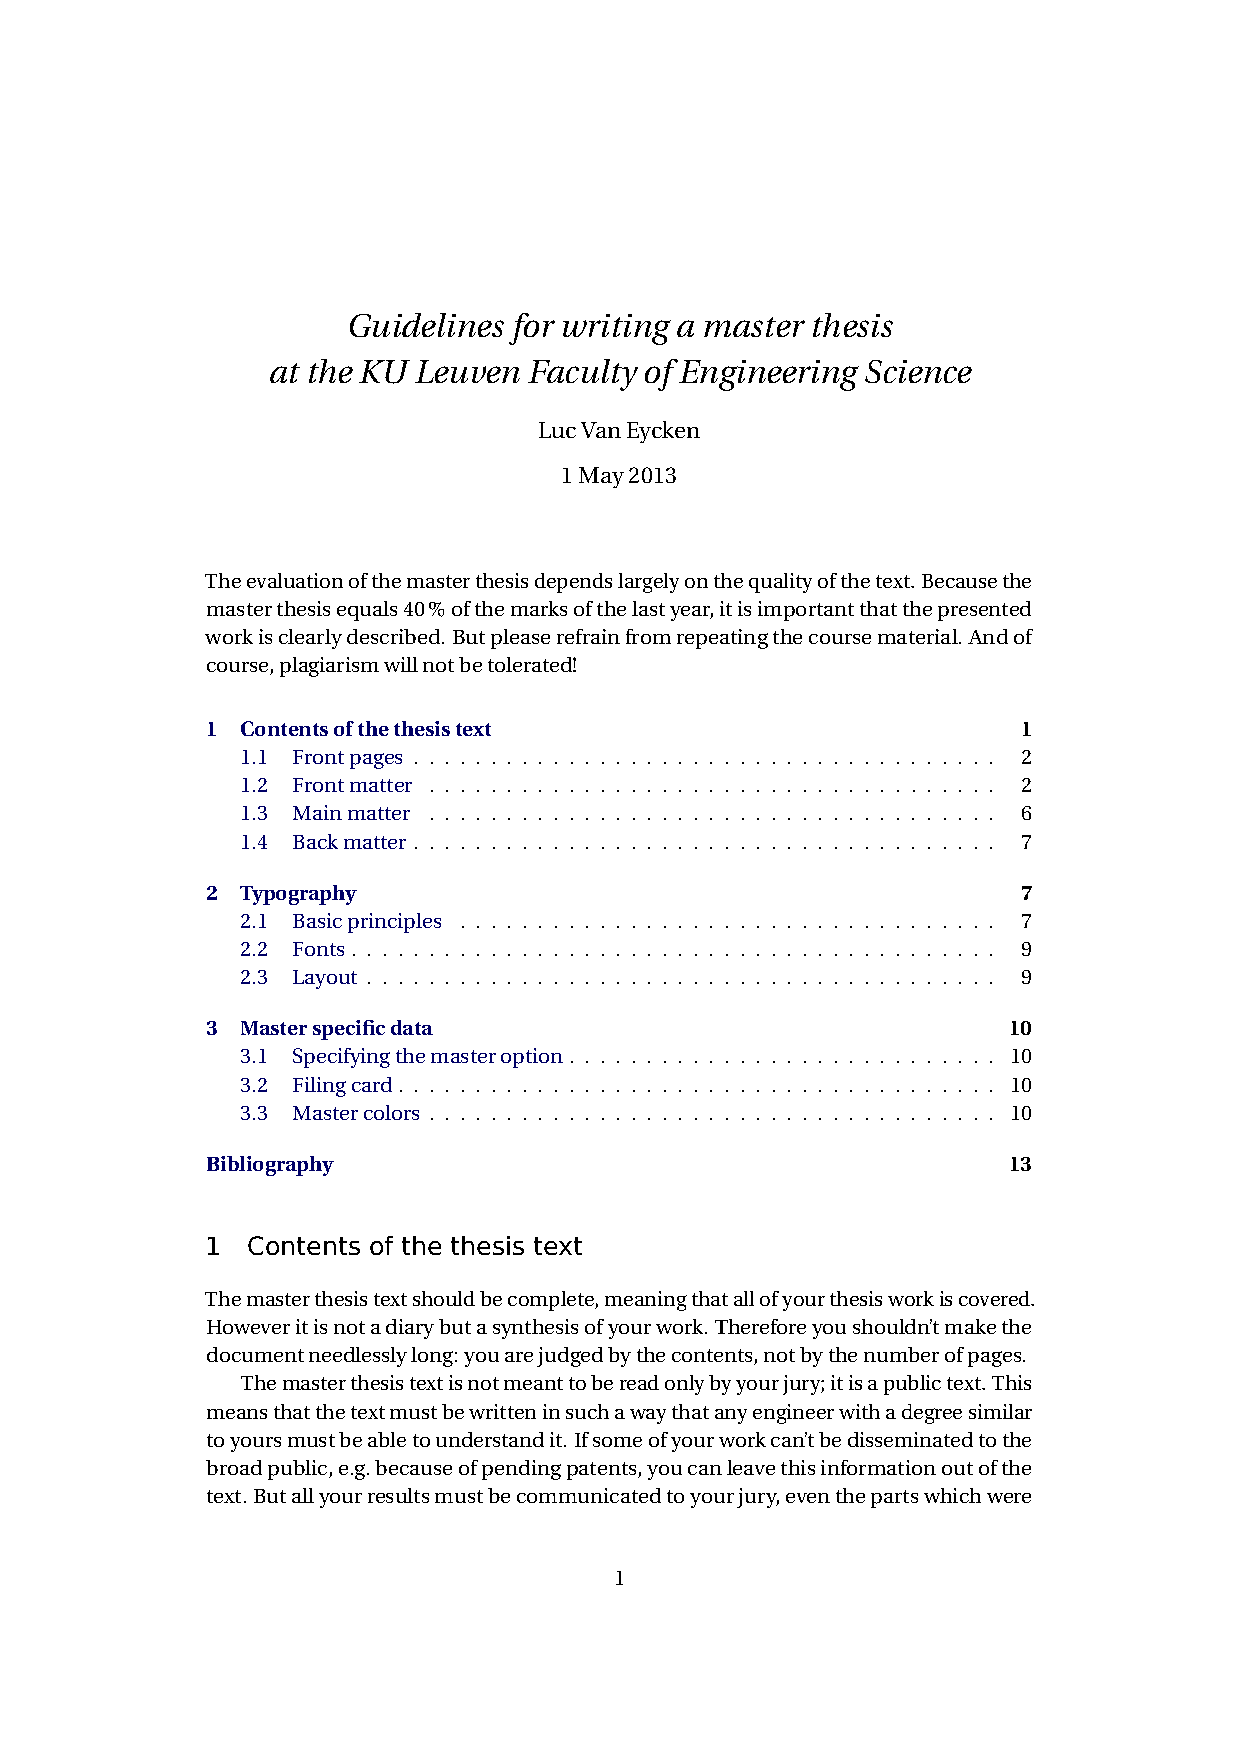
\includepdf[pages=-]{guidelines_thesis.pdf}
%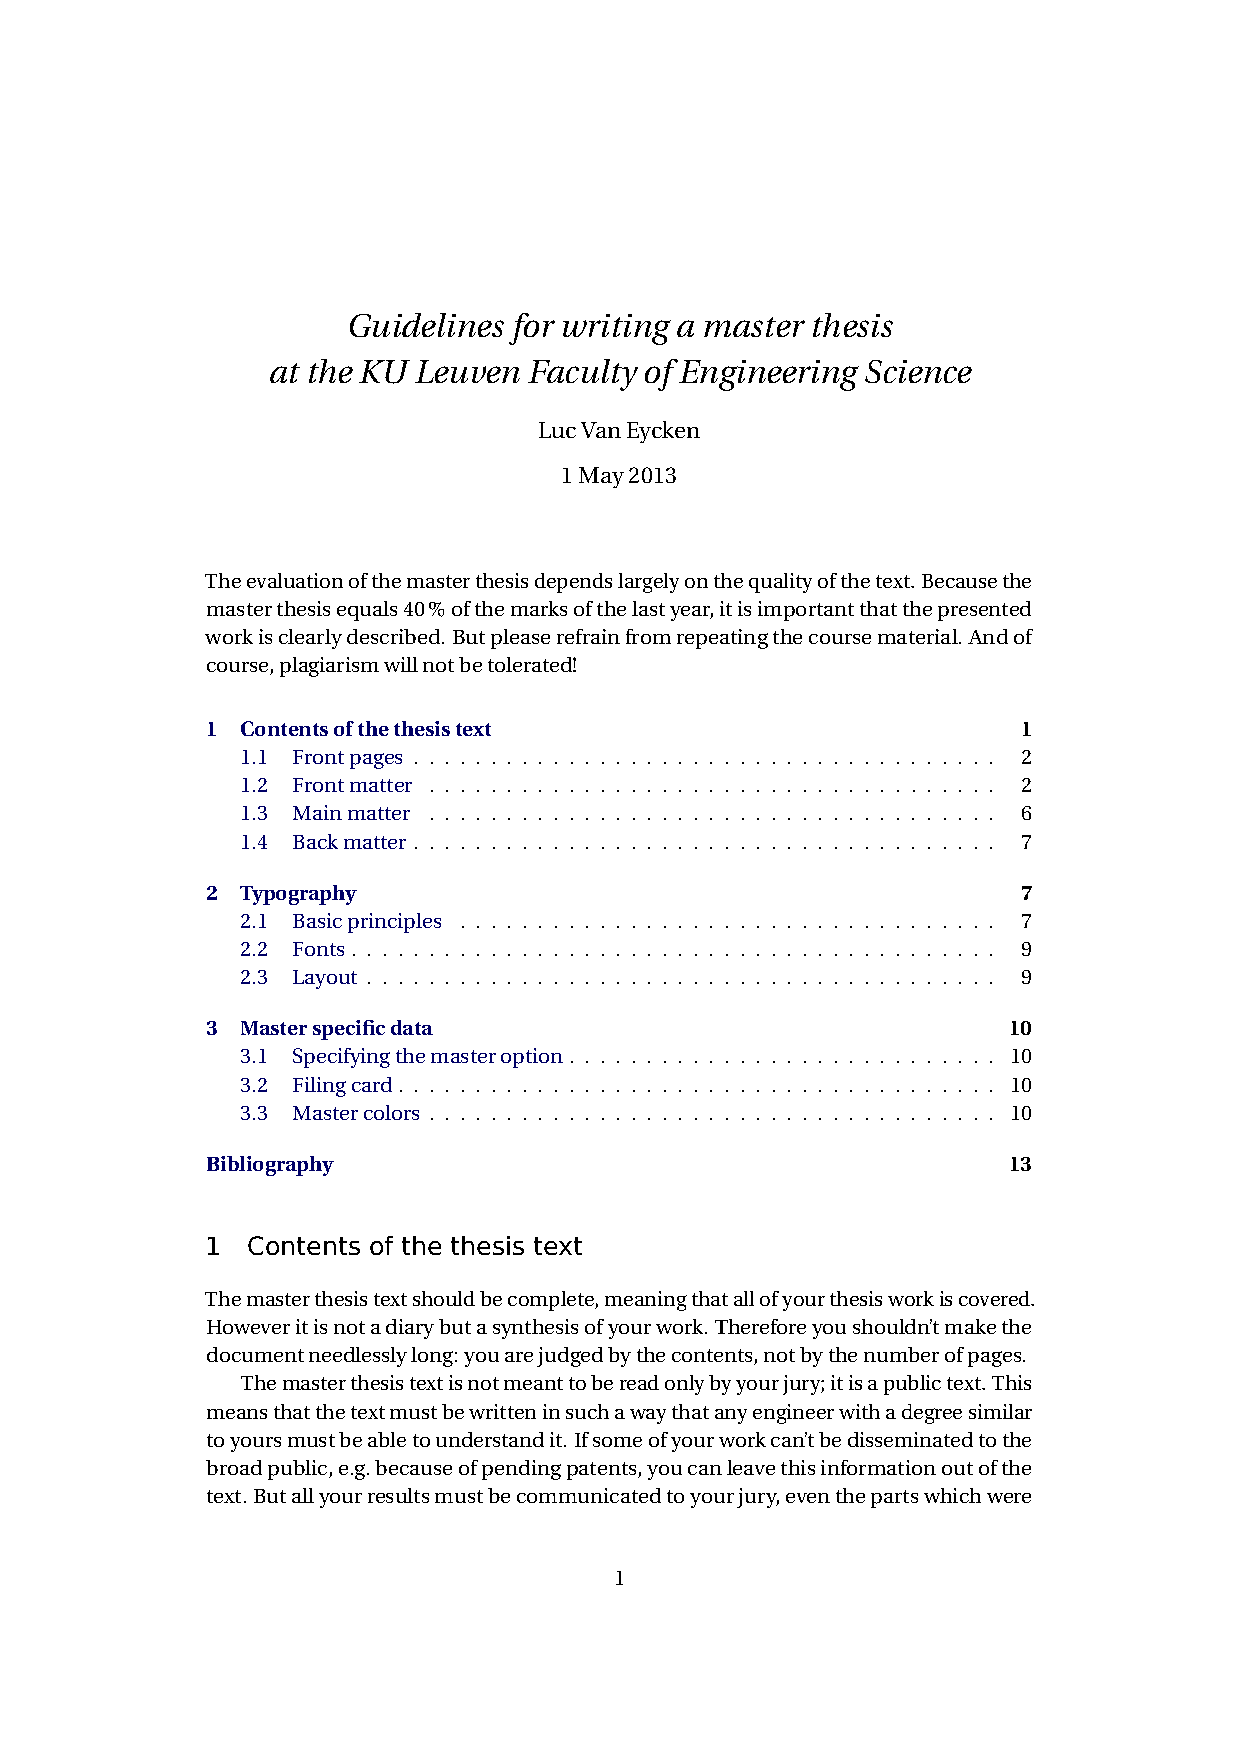
\includepdf[pages={1-2}]{guidelines_thesis.pdf}
%\includepdf[pages=-]{loonjobatprofielvoorbudgetgebruikt.pdf}

%\chapter{bijlage 2}

%\chapter{De eerste bijlage}
\label{app:A}
In de bijlagen vindt men de data terug die nuttig kunnen zijn voor de
lezer, maar die niet essentieel zijn om het betoog in de normale tekst te
kunnen volgen. Voorbeelden hiervan zijn bronbestanden,
configuratie-informatie, langdradige wiskundige afleidingen, enz.

In een bijlage kunnen natuurlijk ook verdere onderverdelingen voorkomen,
evenals figuren en referenties\cite{h2g2}.

\section{Meer lorem}
\lipsum[50]

\subsection{Lorem 15--17}
\lipsum[15-17]

\subsection{Lorem 18--19}
\lipsum[18-19]

\section{Lorem 51}
\lipsum[51]

%%% Local Variables: 
%%% mode: latex
%%% TeX-master: "masterproef"
%%% End: 

% ... en zo verder tot
%\chapter{De laatste bijlage}
\label{app:n}
In de bijlagen vindt men de data terug die nuttig kunnen zijn voor de
lezer, maar die niet essentieel zijn om het betoog in de normale tekst te
kunnen volgen. Voorbeelden hiervan zijn bronbestanden,
configuratie-informatie, langdradige wiskundige afleidingen, enz.

\section{Lorem 20-24}
\lipsum[20-24]

\section{Lorem 25-27}
\lipsum[25-27]

%%% Local Variables: 
%%% mode: latex
%%% TeX-master: "masterproef"
%%% End: 


\backmatter

%for bibtex
% Na de bijlagen plaatst men nog de bibliografie.
% Je kan de  standaard "abbrv" bibliografiestijl vervangen door een andere.
%\nocite{*}
%\bibliographystyle{abbrv}
%\bibliography{referenties}

\chapter{Bibliografie}


%for bibLatex
%\printbibliography[heading=bibintoc,title={Whole bibliography}] %Prints the entire bibliography with the titel "Whole bibliography"

%hiermee worden alle entries getoond, zelfs als ze niet vermeld worden in de tekst.
%\nocite{*}

%Filters bibliography
\printbibliography
\printbibliography[heading=subbibintoc,type=online,title={Sites only}]
\todo[inline]{Gebruikte bronnen en sites nog als bibliografie toevoegen achteraan.}

%\printbibliography[heading=subbibintoc,type=article,title={Articles only}]
%\printbibliography[heading=subbibintoc,type=book,title={Books only}]

%op aparte pagina zo schrijven dan
%\printbibliography[type=book,title={Books only}]
%\printbibliography[keyword={physics},title={Physics-related only}]
%\printbibliography[keyword={latex},title={\LaTeX-related only}]

%\chapter{Index}

\printindex


\end{document}

%%% Local Variables:
%%% mode: latex
%%% TeX-master: t
%%% End:
